\documentclass[output=paper,
modfonts
]{langscibook} 
\bibliography{localbibliography}

\usepackage{tabularx,multicol}
\usepackage{url}
\urlstyle{same}

\usepackage{longtable} % to be able to make the long table in Data span over multiple pages - JP
\usepackage{multirow} % to be able to use the multirow command - needed for Paper 2 tables

\usepackage{langsci-lgr}
\usepackage{langsci-branding}
\usepackage{langsci-optional}
\usepackage{langsci-gb4e}


\makeatletter
\let\thetitle\@title
\let\theauthor\@author
\makeatother

\newcommand{\togglepaper}[1][0]{
%   \bibliography{../localbibliography}
  \papernote{\scriptsize\normalfont
    \theauthor.
    \thetitle.
    To appear in:
    Change Volume Editor \& in localcommands.tex
    Change volume title in localcommands.tex
    Berlin: Language Science Press. [preliminary page numbering]
  }
  \pagenumbering{roman}
  \setcounter{chapter}{#1}
  \addtocounter{chapter}{-1}
}

\newcommand{\bari}{\ipabar{\i}{.5ex}{1.1}{}{}}
\newcommand{\notipa}[1]{\textnormal{#1}}

\newcommand{\agre}{\textsc{agr}-\ol{eene}}

\renewcommand{\emph}[1]{\textit{#1}} % resetting a setting from ling-macros-modified (I think?)

% forest settings to make compact but (mostly) straight-spined trees:
\forestset{
fairly nice empty nodes/.style={
            delay={where content={}{shape=coordinate,for parent={
                  for children={anchor=north}}}{}}
, angled/.style={content/.expanded={$<$\forestov{content}$>$}}
}}

\forestset{sn edges/.style={for tree={parent anchor=south, child anchor=north}}}

\newcommand{\bex}{\begin{exe}}
\newcommand{\fex}{\end{exe}}

\newcommand{\bxl}{\begin{exe}}
\newcommand{\fxl}{\end{exe}}

\newcommand{\ix}[1]{\textsubscript{#1}}
\newcommand{\alert}[1]{\textbf{#1}}
\newcommand{\ol}[1]{\textit{#1}}


\newenvironment{context}{\begin{quote}%
			\bfseries Context: \\%
			\mdseries\slshape }%open environment
			{\end{quote}}%close environment




			\usetikzlibrary{shapes,arrows,positioning,decorations,decorations.pathmorphing,intersections}
\forestset{
nice empty nodes/.style={
    for tree={calign=fixed edge angles},
    delay={where content={}{shape=coordinate,for siblings={anchor=north}}{}}
},
}

\definecolor{dark-gray}{gray}{0.3}

%\usepackage{dingbat,pifont}


%%%%%%%%%%%%For arrows%%%%%%%%%%%%%

\newcommand\Tikzmark[2]{%
  \tikz[remember picture]\node[inner sep=0pt,outer sep=0pt] (#1) {#2};%
}
\NewDocumentCommand\DrawArrow{O{}mmmmO{3}}{
\tikz[remember picture,overlay]
  \draw[->,line width=0.8pt,shorten >= 2pt,shorten <= 2pt,#1]
    (#2) -- ++(0,-#6\ht\strutbox) coordinate (aux) -- node[#4] {#5} (#3|-aux) -- (#3);
}
\NewDocumentCommand\DrawDotted{O{}mmmmO{3}}{
\tikz[remember picture,overlay]
  \draw[->,line width=0.9pt,dotted,shorten >= 2pt,shorten <= 2pt,#1]
    (#2) -- ++(0,-#6\ht\strutbox) coordinate (aux) -- node[#4] {#5} (#3|-aux) -- (#3);
}
\NewDocumentCommand\DrawLine{O{}mmmmO{3}}{
\tikz[remember picture,overlay]
  \draw[line width=0.8pt,shorten >= 2pt,shorten <= 2pt,#1]
    (#2) -- ++(0,-#6\ht\strutbox) coordinate (aux) -- node[#4] {#5} (#3|-aux) -- (#3);
}
%%%%%%%%%%%%%%%%%%%%%%%%%%%%%%%%%%%%%


\newcommand{\baru}{ʉ}
\newcommand{\baruH}{\'\baru}
\newcommand{\baruL}{\`\baru}

\newcommand{\ep}{ε}
\newcommand{\epH}{\'\ep}
\newcommand{\epL}{\`\ep}

\newcommand{\schwa}{ə}
\newcommand{\schwaH}{\'ə}
\newcommand{\schwaL}{\`ə}

\newcommand{\oo}{ɔ}
\newcommand{\ooH}{\'\oo}
\newcommand{\ooL}{\`\oo}

\newcommand{\ds}{\ꜜ}

\newcommand{\ch}{t͡ʃ}
\newcommand{\dz}{d͡ʒ}

\newcommand{\tgl}{ʔ}

%shortcuts for the complementizers
\newcommand{\mbuL}{mb\baruL}
\newcommand{\mbuHL}{mb\baruH\baruL}
\newcommand{\mbuLH}{mb\baruL\baruH}
\newcommand{\la}{lá}
\newcommand{\nda}{ndà}

\newcommand{\tsc}[1]{\textsc{#1}}
\renewcommand{\textscb}{ʙ}
\newcommand{\ipa}[1]{#1} %disable IPA

 
\title{Contact Languages}

\author{%
 Danae Perez\affiliation{Zurich University of Applied Sciences}
}




\abstract{
This chapter gives an overview of different processes of contact-induced language change that lead to the emergence of new languages. The principal focus lies on the emergence of pidgin and creole varieties. The first sections outlines the most prominent theoretical approaches that have guided the field since the early 20th century, showing that very different approaches to contact languages have been proposed, and that only a combination of them may account for all individual cases. The next section focuses on the grammatical processes involved in contact-induced grammaticalization, often referred to as “creolization”, and points out that processes of simplification and complexification as well as calquing happen on all levels of grammar. The last part lists the factors that determine the emergence of new languages. They include a wide range of determiners, from psycholinguistic conditions of incomplete L2 acquisition to the sociocultural setting. The chapter ends in claiming that within the field of contact linguistics, the study of the emergence of new languages may be the most interdisciplinary one.
}

\begin{document}
\maketitle


\section{Introduction}

The present chapter outlines the processes triggered by intense and prolonged contact between speakers of different, and usually unrelated, languages that ultimately gives birth to new languages. Newly emerged contact languages can be found all around the globe. Most of the contact languages known today have emerged over the past five centuries as a consequence of the spread of colonizing nations into new territories. They are therefore based on European colonizer languages, though also non-Indo-European-lexified contact languages exist, such as those based on Bantu in Southern Africa \parencite{apics}. \cite{meshtrie2017slavery} broadly distinguishes between two different classes of contact languages: koinés, or leveled dialects, on the one hand, and pidgins and creoles, on the other. The former arise in colonization settlements involving indentured work where larger and linguistically rather homogeneous communities transplant and restructure their related varieties into a new one. The latter usually emerge when speakers of different languages come into contact and need to find a common code, which often occurred in contexts of slavery or trade. While the former are described in \cite{ruchetal_tv} and \cite{jeszenskyetal_tv}, 
the latter are the topic of the present chapter.

The interdisciplinary study of contact languages is a rather new field within linguistics. Until the late 19th century, most linguists studied standard languages from a philological perspective. They saw languages as deteriorating in terms of quality and purity, while only standard forms were considered worthy of retention and study. The pioneer to first look at non-standard varieties was the Austrian Hugo Schuchardt. He noticed that travelers in different corners of the Portuguese-speaking world observed similar non-standard language patterns and sent out questionnaires to inquire about these patterns. His revolutionary interest in contact varieties induced other linguists to pay more attention to the processes triggered by language contact, yet the decades to follow did not bring much innovation to the field. Given the mainly oral character of contact languages and their commonly rather low social status, the first approaches to these language varieties were cautious and descriptive only, and the documentation was slow. In fact, to date the documentation of creole varieties is difficult due to their social marginalization and lack of written records \citep[cf.][]{garrett2006contact}.

Contact languages emerge in a wide range of different sociolinguistic contexts with a myriad of different combinations of languages involved. The processes at stake and the linguistic outcome differ from case to case. As a result of this diversity, no unanimously acknowledged typological definition of a pidgin or a creole has so far been proposed, and certain scholars
\citep[e.g.][]{mufwene2008language} hold that creolization is, in fact, an exclusively social process. In general terms, a pidgin language can be defined as a limited code that has no native speakers because it results from the communication between speakers of different languages in one specific domain only, such as trade. It usually contains lexical elements of all the languages involved, and it is lexically and morphologically limited to the needs of the speakers in this one specific domain. The TMA (Tense-Mood-Aspect) system, for instance, is often based on a low number of individual and invariant markers stemming from adverbs present in any of the involved languages, and the use of prepositions or morphological processes, such as reduplication, is low \citep{bakker2008pidgins}.

As opposed to such reduced codes, creoles are fully developed languages. They are fully functional for their speech community within their respective context and acquired natively by community members. In many cases, creoles develop out of pidgins as their new native speakers expand them stucturally and lexically. Nigerian pidgin, for example, was originally a pidgin and has now evolved into a “pidgincreole” with millions of speakers \citep{bakker2008pidgins}. This pattern, however, does not always apply; some creoles are said to have developed in the opposite direction, i.e. they have become more different from the lexifier over time \citep{chaudenson2001creolization}. Structurally, creoles display a vast array of different features. This makes it difficult to provide a universal definition. In general, they are rather isolating languages that make use of grammaticalized TMA markers rather than affixation, and they mostly have an SVO word order. The main proportion of their lexicon stems from the lexifier language, while grammatical structures have resulted from different origins and processes of language change \citep{bakker2008pidgins, bartens2013creole}.

In fact, the endeavor of finding a universally applicable synchronic definition of creoles continues to challenge linguists. They seek to classify contact languages on the basis of a feature-based typological comparison. McWhorter \cite{mcworther1998identifying, mcworther2005defining} proposed the “prototypical creole” to be distinguishable from non-creoles on the basis of three coexisting features, namely 1) the lack of inflectional affixation, 2) the lack of tonal distinctions, and 3) the lack of non-compositional derivation. \cite[5]{mcworther2005defining} holds that these features are present in all creoles because they are “the world’s newest languages” as opposed to “older” languages that have evolved over several millennia and had the time to develop combinations of these features. Along the same lines, Bakker and Daval-Markussen (2011) crystallized four features that seem to set creole languages apart, and \cite[14]{daval2014first}, in his comparison of creoles with non-creoles proposes 1) an indefinite article based on “one”, 2) no tense-aspect inflection, 3) the presence of a negative particle, and 4) the presence of possessive structures based on “have” as the typical creole features. His focus, however, lies on English-based creoles.

Given this structural diversity across creole languages and the unresolved challenge of defining them synchronically, certain linguists claim that it is their social history of language contact, rather than a set of structural features, that defines creole languages as such \citep[cf.][]{mufwene2000creolization, chaudenson2001creolization, mufwene2001ecology, degraff2005linguists, mufwene2008language}.

\cite[15]{bakker2017key}, however, specifies that “a creole is in principle a language associated with certain sociohistorical events, but if the linguistic structures after such events do not conform to ideas about what a creole language is supposed to be like, we do not call a language a creole”. A synchronic typological definition of creoles is thus needed. Yet, as Section \ref{approaches} will show, the definition, the classification, and at times even the emergence of creoles are far from resolved.
	
The aim of this chapter is to provide an overview of current trends in the field of creolistics, and to point out their importance within the discipline of contact linguistics. I will first give an overview of the theoretical and methodological approaches to these varieties and present proposals for a universal definition of creole languages in Section \ref{approaches}. In Section \ref{patterns}, I will look at patterns of change and how they have been explained. Section \ref{factors} describes the determining linguistic and extralinguistic factors, while the discussion in Section \ref{conclusion} critically looks at possible future directions the field may take.

\section{Approaches, models, and methods} \label{approaches}

The fact that similar features are attested across different contact varieties despite the typological diversity among their input languages is intriguing. Among these similarities are the three general typological features proposed by \cite{mcworther1998identifying} - see above, in addition to other, more specific ones, such as the presence of independent-locative and TMA markers. It has been argued that these shared features are the result of basic varieties spreading in the course of European colonization. McWhorter’s Afrogenesis Hypothesis \citep{mcworther2000missing}, for instance, claims that all Atlantic creoles have one single origin on the West African coast where basic pidgins used by slave traders provided the structural basis for all the future creoles in the region. With regard to English-lexifier creoles, such as West African and Caribbean varieties, he bases his argument on six parallel features found in many Atlantic varieties of English, and he argues that the origin of that basic code was the Cormantin trade fort in Ghana from where its speakers were shipped into the New World. Among these six features is the locative copula \emph{de}, derived from English \emph{there}, which is attested in numerous English-lexifier creoles between Nigeria and Belize. \cite{huber1999atlantic}, however, doubts that the Ghanaian coast was the cradle of Atlantic English-based creoles and suggests a locale in the New World as the point of departure of such an ancestor variety. Along the same lines, \cite{baker1999investigating} proposes an “embryonic variety” of English to have spread from St Kitts in the Lesser Antilles into the wider region. West African English-lexifier creoles are also claimed to constitute a linguistic area, and their shared structures stem from both a common Krio substrate as well as similar adstrate influences \citep{yakpo2017towards}.

Comparable claims of diffusion were also raised about Iberian-lexified contact varieties. \cite{ferraz1987portuguese} argued in favor of the relatedness of the Portuguese-based Gulf of Guinea creoles due to a common origin, and more recently, \cite{hagemeijer2011gulf} supported Ferraz’ assumption claiming that a basic variety spread from the central administration in São Tomé to other locales in the Gulf of Guinea archipelago. With a wider, cross-Atlantic focus, \cite{jacobs2009upper} argues in favor of a Capeverdean origin of Papiamentu on the basis of an analysis of the lexicon; and in fact, Capeverdean creole also seems to have provided some of the core vocabulary of English-lexified Saramaccan in Suriname and Guinea-Bissau Creole Portuguese \citep{jacobsetal2016relevance}. \cite{mello1996genesis} and \cite[29]{lipski2005history} assume that Brazilian Vernacular Portuguese is likely to have a reduced Portuguese-based code as a substrate that was used in the pan-Atlantic slave trade. And while \cite{lucchesietal2009portugues} contradict this claim holding that creoloid varieties of Afro-Portuguese mushroomed individually in different locales of Brazil, \cite{perez2015traces} rather follows the former hypothesis proposing that such a basic contact variety of Portuguese may have been one of the substrates to Afro-Yungueño Spanish spoken in as remote a location as the Bolivian Andes. This shows that the Atlantic, as a linguistic area, provides intriguing evidence to assume the diffusion of stable features over the past five centuries. The particular linguistic outcome in each location, however, differs and depends on the individual history of, and input to, the contact language.

As opposed to such claims of diffusion, the universalist approach proposes that certain patterns found in most creoles are universally human and thus the result of universal processes of language evolution. Bickerton’s seminal \emph{Language Bioprogram Hypothesis} \citep{bickerton1981roots} claimed that universal, i.e. innate, processes of language acquisition are at stake in the evolution of pidgins and creole languages. His argument is that the limited input the children receive from their pidgin-speaking parents needs to be expanded, and this expansion follows universal psycholinguistic patterns. This explains, according to Bickerton, why many creoles typically have twelve diagnostic features in common. Even if these features have been declared to be insufficiently diagnostic and Bickerton’s Language Bioprogram Hypothesis is rarely adduced in the debates around creole genesis today, it did significantly determine the directions of the field. Also \cite{mcworther1995sisters} and \cite{parkvall2000out}, among others, argue that creoles have emerged from basic pidgins that were expanded by their first generations of native speakers according to universal parameters.

This comparative approach has been fostered by elaborate feature sets that have been made available for comparative studies. Among them, the collection of morphosyntactic structures provided by \cite{holmetal2007} was pioneering as it compared creole structures across the Atlantic and the Pacific. Their work laid the foundation for the Atlas of Pidgin and Creole Structures (APiCS, \citealt{apics}), which describes 130 features in 76 contact languages. This recent availability of large comparative datasets (also the World Atlas of Language Structures, \citealt{wals}) thanks to documentational efforts, added to the use of computational methods, has made large-scale comparative studies to measure the relative typological distance between varieties possible. \cite{bakkeretal2013creoles} compared features of 188 languages (153 non-creoles, 34 pidgins and creoles, and the artificial language Esperanto) in a phylogenetic Neighbornet Splitstree diagram. It visualizes how languages cluster according to their typological similarities. They found that creoles cluster as a group, which they take as evidence for seeing creoles as representing their their own typological class, rather than seeing them as an offspring of their lexifiers. They conclude “that creoles (and pidgins, for that matter) are typologically distinct from the languages of the world” \citep[39]{bakkeretal2013creoles}.

These studies, however, have received considerable resistance. \cite{fonsing2017creoles} reevaluates the study by \cite{bakkeretal2013creoles} and concludes that, depending on the selection of features, creoles do not necessarily cluster. \cite{blasietal2017grammars} hold that overall, European lexifier structures and West African substrate structures are transmitted “robustly” in contact settings, thus suggesting that a previous pidgin state in their history is unlikely, while the transmission of structures existing in the input varieties is stronger. This goes against seeing creole languages as constituting a language class of their own, and it is in line with earlier claims seeing creoles as the continuation of normal processes of language change that all languages undergo \citep[e.g.][]{mufwene2008language}.

Still, the phylogenetic quantitative comparison of varieties has contributed new and useful insights on the degree of creolization that certain varieties undergo. This, in turn, is useful to determine how languages can be classified either as creoles or dialects of their lexifiers. \cite{perezetal2017afro} compared 24 post-colonial dialects of Spanish, standard Spanish, and contact varieties of Spanish on the basis of 72 features with the goal of classifying Afro-Hispanic varieties. The typological status of Afro-Hispanic varieties as either dialects of Spanish, creoles, or “semi-creoles” \citep[cf.][]{holm2004languages} is still subject to debates, and the authors therefore aimed to determine where these varieties would appear in a Splitstree diagram. The results showed that creoles and dialects of Spanish cluster on the two opposite ends of the diagram, suggesting maximal typological difference between them, while Afro-Hispanic varieties indeed appear somewhere in-between these two clusters. The authors hence conclude that the history of intense language contact is reflected in the typological profile and becomes visible in the Splitstree diagram. Along the same lines, \cite{perez2017from} assesses the status of Afro-Yungueño, an underresearched creoloid variety of Spanish spoken in the Bolivian highlands whose typological status had not yet been determined unanimously \citep[cf.][]{perezetal2017afro}. This study compares 60 features from APiCS, WALS, and Spanish and Portuguese dialectology in 21 varieties, i.e. Iberoromance-lexified creoles, contact varieties of Spanish and Portuguese, as well as standard Spanish and Portuguese. The goal is to better understand how closely related or distant Afro-Yungueño is from other related varieties, and whether it rather belongs to the creole type or not. Figure \ref{CreoleNN} shows that that Afro-Yungueño appears in the cluster of creoles on one end, while dialects and contact varieties of Spanish and Portuguese cluster at the opposite end of the diagram. This leads to the conclusion that Afro-Yungueño is typologically as distant from its lexifier as other creoles and should thus be classified as a creole. In general, these feature-based analyses and large-scale comparisons of creole languages with non-creole languages are useful to better understand the typological profile that defines creoles as such.\\

\begin{figure}[h]
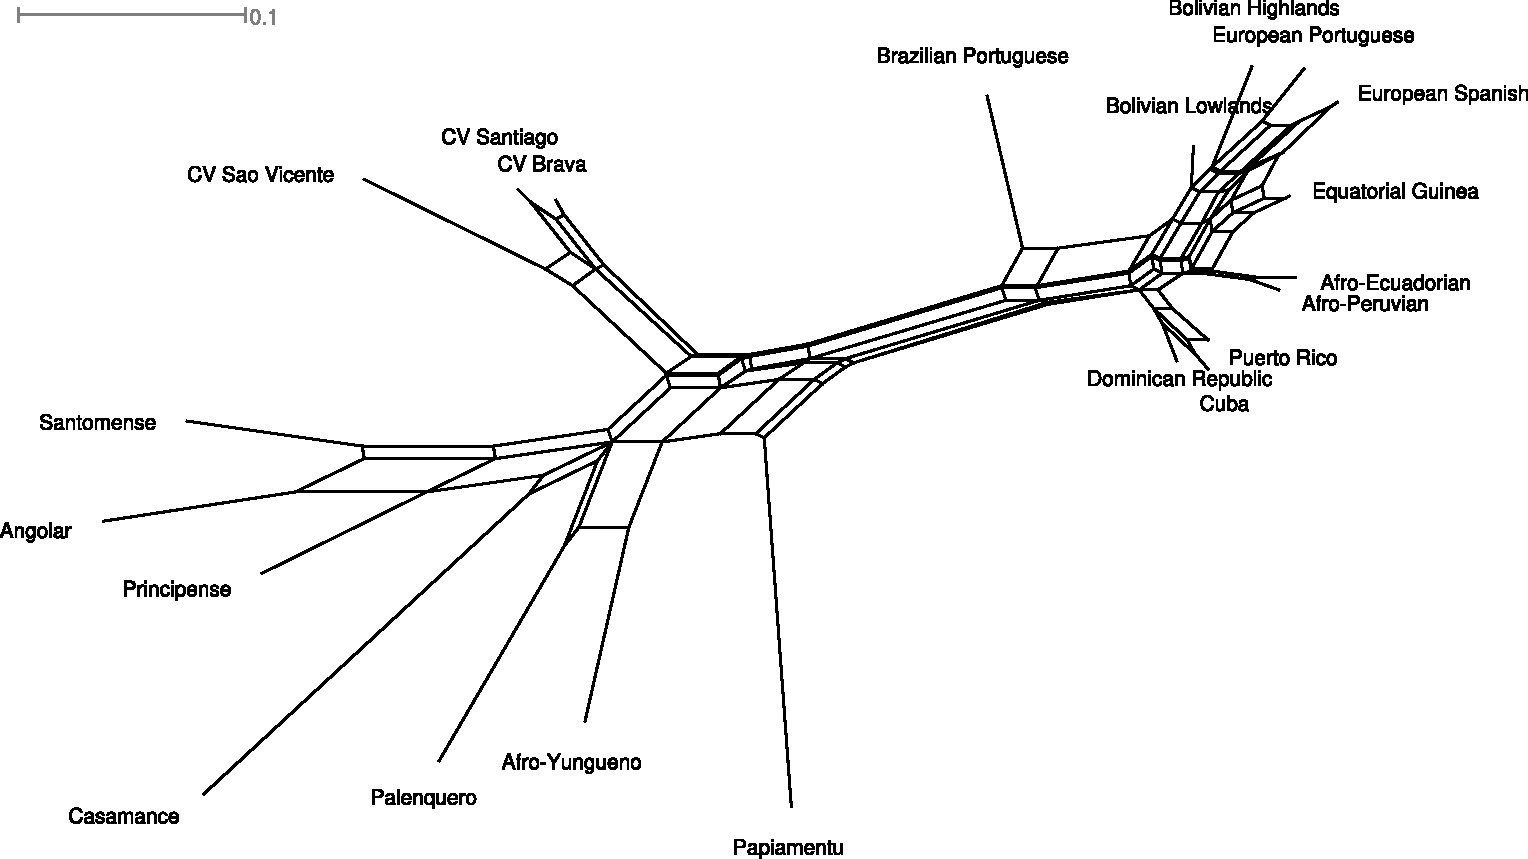
\includegraphics[width=\textwidth]{CreoleNN.pdf}
\caption{Comparison of Spanish and Portuguese varieties and contact languages on the basis of 60 features} \label{CreoleNN}
\end{figure}

\noindent Given that creoles are highly contextualized languages and intimately influenced by the ecology in which they emerge \citep{jourdan2008cultural}, these large-scale comparisons still heavily rely on in-depth and ethnographically informed data sets.

One of the shortcomings of these comparative studies is that they suggest homogeneous varieties. There is, however, considerable variation found in individual speakers, which challenges the description and classification of creoles. In most Caribbean societies, for instance, basilectal creoles coexist with their same-lexifier acrolectal standard variety, and speakers switch between the basilect and the acrolect. This situation has provided the foundation for claims holding that speakers and their language use can be located on a continuum between the creole on one end and the acrolect on the other. This model is called the (post)creole continuum \citep[cf][]{decamp1971toward}. This model was tested on different varieties in a variationist way; Patrick’s \citeyear{patrick1999urban} variationist study, for instance, explains that speakers are more likely to display the simultaneous use of certain Jamaican Creole features together with Jamaican English features depending on their level of schooling and/or professional status. The presence or absence of creole features in a bilingual individual’s speech is thus structured and predictable, which he takes as evidence in favor of such a continuum existing not only in society, but also within individual speakers. Studies like \cite{patrick1999urban} also show how useful variationist approaches to creoles are, particularly since creole speakers often display a particularly high level of variation.

Others, however, reject the continuum approach and hold that Caribbean countries rather represent diglossic societies \citep[cf.][]{ferguson1959diglossia}, since the languages involved have different social statuses and fulfill different functions. In these societies, the creoles represent the low variety L, while their superstrate or acrolect – usually the lexifier – represents the high variety H. Full access to the H variety is usually restricted to members of the upper classes \citep[cf.][]{winford1985concept}. Speakers thus switch between languages, rather than moving along a continuum of the one and same language between the acrolect and basilect. \cite{devonish2003language} expands the original definition of diglossic societies to what he defines as cases of “conquest diglossia”, because a non-native variety is imposed forcefully. \cite{winford1985concept} claims that Caribbean creoles and their coexisting standard languages belong to “two conflicting sets of underlying values”, because in addition to them being used in different contexts, the values attached to each code are highly controversial. On the one hand, the creoles are still seen as inferior and uncivilized codes, and sometimes even as not being legitimate languages, i.e. they are of low prestige in their respective societies \citep[cf.][]{rickfordetal1985symbol, patrick2008jamaican, kouwenbergetal2011linguistics}. On the other, creoles as the vernaculars spoken by the majority of the population have also been argued to be of covert prestige, because they have a “high affective or solidarity value” \citep[259]{rickfordetal1985symbol}. This means that in formal contexts, in which the use of a standard language may seem more appropriate, creoles can have an “anti-formal effect” that is positively valued \citep{allsopp1996dictionary}. This was also reported in analyses of style shifts among educated speakers of Jamaican creole and English, for instance, who make use of the two codes as a subtle narrative strategy, e.g. in direct speech, as well as to express group allegiance (\citealt{deuber2009english}; cf. also \citealt{patrick2008jamaican} and for email data, see \citealt{hinrichs2006code}).

In fact, \cite{lepageetal1985acts}, in their pioneering study on language and identity, claimed that language choice is always socially marked, and that the preference for one language over the other, especially that of a creole over its more prestigious lexifier, constitutes an “act of identity”. They argue that language “has the extra dimension in that we can symbolize in a coded way all the other concepts which we use to define ourselves and our society” \citep[247-248]{lepageetal1985acts}. In multilingual societies, such as West Africa \citep{yakpo2017towards} or the Philippines \citep{leshoetal2013sociolinguistic}, however, the case may again be different, since the creole may even be of higher status, as is the case with Chabacano in the Philippines, or the creole may be the only language speakers of different linguistic backgrounds have in common. Creole-speaking societies thus offer fascinating insights into various social aspects of language use, and their study was groundbreaking in many respects and pushed sociolinguistics to explore new areas.

\section{Patterns} \label{patterns}

As seen so far, pidgins and creoles are the result of language change triggered by intense language contact. When a new language emerges as the result of the contact between speakers of languages, each of the input languages plays its own role. The language that is (often forcefully) adopted as the target language is called the lexifier language because it provides most of the lexical material to the new language. The languages originally spoken by first-generation speakers are called substrates, while the languages that coexist alongside the new language are adstrate languages. The superstrate language, finally, is the socially dominant language, which is often the same as the lexifier language, as in Jamaica (Jamaican Creole and English) or Cape Verde (Cape Verdean Creole and Portuguese), but it can also be a different language, as in Equatorial Guinea, where Pichi is English-lexified and its superstrate is Spanish \citep[cf.][]{yakpo2017towards}. All these languages provide different proportions of grammatical structures to the new language, yet overall, the substrates are most relevant in the early stages when second-language speakers bring in their first-language structures, while adstrates and superstrates determine ongoing change in contact languages after the contact language has been established.

The changes at the root of the emergence of new languages entail grammaticalization patterns that go beyond short-term accommodation, leveling, and new-dialect formation or code-switching (i.e. the adaptation towards the speech of an interlocutor and other conversation-internal features; see \citealt{ruchetal_tv}), because long-term accommodation may lead to large-scale leveling and the emergence of new forms and norms (cf. e.g. \citealt{kerswill2010contact}). Moreover, while pidgins are always limited to the domain in which they are used, the emergence of a creole, i.e. a new native and fully functional language, often comes along with the loss of the speakers' original L1s and the involved substrate languages \parencite[see]{karnopp_tv}. Finally, in the case of the movement of larger groups, features and patterns spread geographically from one locale to the next and may come to form a linguistic area \parencite[see]{gijnetal_tv}.
The interdisciplinary study of the emergence of new languages, commonly called creolistics, may hence be the discipline that brings all the other branches of language contact together.

Parts of the grammar of a creole is composed of structures that were calqued from the lexifier, the substrate, or an adstrate language, while other structures result from internal processes of innovation and grammaticalization and adult L2 acquisition \citep{bakker2008pidgins,bartens2013creole}. Given the rapid growth of a new system, change in contact languages happens at a high pace. Winford \citep[in][]{baptista2017competition} holds that contact-induced language change is faster than internally-motivated change. The process of the emergence of pidgins and creoles is generally described as creolization. Certain scholars who rather subscribe to the universalist approach holding that creoles stem from pidgins, however, distinguish between pidginization, i.e. the extreme reduction of grammar due to “broken transmission”, and creolization, i.e. the subsequent expansion of grammatical structures that comes along with nativization \citep[e.g.][3,9]{parkvall2000out}. The early “reduction” \citep{bakker2008pidgins} or “simplification” \citep{mcworther2011why} of a variety to a pidgin includes processes that reduce the morphosyntactic complexity of languages, such as the loss of irregular structures, and an overall trend toward isolating or analytic patterns \citep{trudgill2011sociolinguistic}. This early phase of pidginization is labeled “jargonization” by \cite[50]{good2013typologizing}. Based on the assumption that creoles have developed from early pidgins, creole grammars have been claimed to be overall simpler than non-creole (i.e. older) grammars \citep{mcworther2011why}. Taking this idea as a point of departure, \cite{parkvall2008simplicity} compares the complexity of 155 languages on the basis of 53 features and finds that creoles indeed appear at the end of the complexity scale. He explains that this has to do with their age, because pidgins and expanded pidgins have not yet had the time to develop more complex systems (\citeyear[283]{parkvall2008simplicity}).

It is important to note, however, that by complexity most linguists refer to morphological complexity. On other levels, such as phonology, creoles tend to become more complex than their lexifiers. \cite{perezetal2019relevance} show that unusual voice patterns, such as breathy voice to convey pragmatic meaning, can emerge in contact scenarios. Processes of creolization thus affect all levels of linguistic structures.

In general terms, and for the sake of simplicity, creolization can be seen as contact-induced grammaticalization that occurs on all linguistic levels to the degree of typologically removing the new language from all the languages that were originally involved. This means that creolization is large-scale grammaticalization that gives birth to a typologically distinct language. \cite{detges2000two} and \cite{bruyn2008grammaticalization} claim that creolization is a type of language change that is particular to creoles. In many French-based creoles, for example, an independent marker fini (from French finir ‘to finish’) is found, and its meaning today includes the reference to time as COMPLETEDNESS as well as intensification, in addition to the original meaning of the verb ‘to bring to an end’, as in Mauritian Creole French in Example (\ref{MCF}) and in Haitian Creole French in Example (\ref{HCF}):

\ea \textnormal{Mauritian Creole French. \citep[139]{detges2000two}}\\
\label{MCF}
\gll Mon Dié moi \textbf{fini} bête\\ 
My God \textsc{1sg} \textsc{int} stupid\\
\glt ‘My God, I’m \textbf{completely} stupid!’ 
\z

\ea \textnormal{Haitian Creole French, \citep[140]{detges2000two}}\\
\label{HCF}
\gll M \textbf{fini} travay-la\\ 
\textsc{1sg} \textsc{compl} work-\textsc{def}\\
\glt ‘I \textbf{finished} the job.’
\z

Also frequent collocations can result in new uses and meanings of certain items \citep{detges2000two}. In Afro-Yungueño Spanish, for example, \emph{límpyu} (from Spanish \emph{limpio} ‘clean’) has come to mean ‘all’, and it can be combined in bi-morphemic constructions, such as \emph{limpyu kosa} ‘all things’ meaning ‘everything’. This item has changed its original meaning due to the frequent collocation of Spanish \emph{todo limpio} ‘all clean’ in expressions such as \emph{¡Cosechen todo limpio!} ‘Harvest all clean!’, which carried the meaning of \emph{todo} to \emph{limpio} \citep[322]{perez2015traces}.

\cite{heineetal2005language} describe the processes involved in contact-induced grammaticalization as the process of linguistic transfer, i.e. the mapping of a source-language structure onto a target language: “Broadly speaking, contact-induced influence manifests itself in the transfer of linguistic material from one language to another” \citep[2]{heineetal2005language}. They specify that the linguistic material involved can be anything from sounds, forms and structures to meanings and combinations thereof. This means that apart from lexical material, also structures can be borrowed (cf. “matter borrowing” versus “pattern borrowing”, \citealt{matras_grammatical_2007}). This may even affect the suprasegmental phonology of contact varieties, since various creoles, such as English-based Saramaccan spoken in Suriname \parencite{good2004tone} and Pichi in Equatorial Guinea \citep{yakpo2018grammar} have been shown to be tone languages due to substrate and adstrate influence from West African tone languages. Also Equatoguinean Spanish and Central African French are said to be tonal \citep{bordaletal2020}.

This focus on source-language structures being mapped on the material of the new language is to a certain extent compatible with the relexification argument, which holds that certain creoles are relexified substrate languages. According to this particular argument, Haitian creole basically consists of Fon transferred on French lexical material \citep{lefebvre1993role}. In a large-scale comparative study of Atlantic creoles of different lexifiers, however, \cite{parkvall2000out} shows that relatively few of the features found in several Atlantic creoles stem from the substrate languages, thus supporting universal processes of pidginization and subsequent creolization to be more relevant than the transmission and calquing of substrate structures.

Still, some linguists contradict this proposal in that “there are no particular linguistic evolutionary processes likely to yield (prototypical) creoles” \citep[63]{mufwene2000creolization}. \cite{mufwene2001ecology} and \cite[80]{mufweneetal2017} hold that it is the individual idiolects, and the cooperation and accommodation between speakers, which ensure constant convergence, thus maintaining stability and uniformity of varieties over time. Accordingly, they follow a rather populational-theoretical approach to language \citep[following][]{croft_explaining_2000} in comparing creolization with processes of competition in living organisms that adapt to the environment in which they are spoken. The process of change is thus determined by the ecological conditions, and \cite{mufwene_colonization_2008} provides the example of Latin’s evolution into the modern Romance languages to show that creoles are gradually restructured varieties of their lexifiers. This aligns with the claim that creoles are the result of the gradual basilectalization of the lexifier because the speakers of each generation only acquire an already restructured code and restructure it anew, thus moving it further away from the lexifier in every generation \citep[cf.][]{chaudenson2001creolization}. The process of change, however, not only occurs vertically from generation to generation, but also horizontally since speakers adjust immediately to new environments and settings (\citealt[19]{mufwene_colonization_2008}, \citealt{clements2018speech}, cf. also \citealt{ruchetal_tv}

). This implies that the outcome of contact-induced language change is determined by the features present in the initial contact scenario as speakers select one feature over the other. According to this view, creoles and other contact varieties should be studied within the discipline of each language family, rather than a language family of its own.

Mixed (or “intertwined”) languages are different. While they also resulted from intense language contact, they are, in fact, less of a melting pot than pidgins and creoles. They usually consist of two source languages and maintain etymologically distinct grammatical categories. The best documented mixed languages are Media Lengua spoken in highland Ecuador and Michif in the area of Winnipeg, Canada \citep{bakker1997language,muysken1997media}. Media Lengua, as an example,  mostly uses Spanish lexemes adapted to Quechuan phonology, and its grammar is Quechuan. Quechua is a concatenating language, and the grammatical categories and suffixes are predominantly taken from Quechua. Example \ref{ex-ML} illustrates this (Spanish lexemes in bold):

\ea \textnormal{Media Lengua, \citep[384]{muysken1997media}}\\ \label{ex-ML}
    \begin{xlist}
       \ex \gll \textbf{Bos}-mu	\textbf{da}-ni-mi\\
You-to	give-1-\textsc{aff}\\
\glt 	‘I give (it) to you.’
      \ex Kan-mu ku-ni-mi (Quechua)\\
      \ex Te (lo) doy a vos (Spanish)
        \end{xlist}
\z

Mixed languages are thus new languages with two clearly distinguishable lexifiers, and the grammatical structures can be assigned to the respective lexifier, rather than resulting from other processes of contact and change. They do display, however, a certain degree of morphosyntactic simplification \citep{mazzolifortcsecondary}.

\section{Factors} \label{factors}

As has become clear throughout the foregoing sections, the processes triggered by language contact are manifold, and any material or structure of a language can be affected by language contact. In fact, given the rapid change that contact languages experience, their evolution is never completed, and different factors may weigh in differently at different points in time. In the emergence of new structures, both intra- as well as extra-linguistic factors are relevant.

From a language-internal perspective, whether and how features are adopted and/or incorporated will mainly be determined by factors such as (non)salience and (non)markedness, because in L2 acquisition, regular and non-salient features are generally more readily adopted and learned than irregular and marked ones. In addition, the frequency of use of features determines their persistence. For example, in the diachrony of a contact language there may be different influences at different stages, which produces the emergence of equivalent forms \citep{baptista2017competition}. The resulting presence (or absence) of variation will determine the course of language change, i.e. whether a feature will persist or change its function or meaning over time \citep[76]{mufweneetal2017}. Mufwene’s \citeyear{mufwene2001ecology} \emph{Founder Principle} holds that the individual languages in contact provide structural features to a feature pool from which speakers draw structures that are in competition with each other. \cite[50]{Aboh_2006} support this argument holding that the feature pool provides the input for the “recombination” of linguistic features in the newly evolving contact language.

Competition is also acknowledged to determine emerging languages on statistical grounds. \cite{batesetal1987competition} hold that as a result of analogical reasoning in the speakers’ minds, the higher frequency of one variant will favor its realization and establishment in the new code. \cite{plag2011creolization} partially agrees with this approach, yet he also objects that competition of features alone does not explain why certain structures are ultimately chosen, i.e. it does not address possible constraints on the selection and transmission of features. He stresses, and thus goes back to earlier universalist approaches, the role of second-language acquisition, during which the simplification of complex structures is crucial \citep[cf. also][]{trudgill2011sociolinguistic}. L2 acquisition is undoubtedly a determinant factor in the emergence of these languages because most creoles start as L2 varieties spoken by a community whose members do not share a common language other than the lexifier. Their divergent use of the lexifier then gives rise to the emergence of new structures in the creole. According to \cite[102]{plag2011creolization}, “L2 processing … provides a principled explanation for feature selection and feature mixing”, because many creole features are also found in early interlanguages (i.e. learner varieties) and thus the result of L2 acquisition by mostly adult speakers. Among the features shared by early interlanguages as well as creole are, among others, the absence (loss) of contextual inflection (e.g. agreement), the presence of possessive pronouns, SVO or SOV sentence structure, or loss/absence of case marking \citep[93]{plag2011creolization}. \cite{baptista2016creole}, however, critiques that Plag’s suggestion – apart from being based on too small a sample – is too simple in that it mostly focuses on the initial stage of creole genesis without being able to account for what happens at later stages. She supports that only a combination of all approaches can ultimately account for the striking similarities as well as differences among creole languages \citep[140]{baptista2017competition}.

Similarly, the frequency of features has been shown to favor the adoption of features, i.e. the more frequent a certain feature is, the more likely it is to “pass the bottleneck” and be integrated into the newly emerging code \citep{good2013typologizing}. These structures that emerged in the initial phase of contact may then still be found centuries later, such as the calquing of substrate structures \citep[e.g.][]{heineetal2005language}. \cite{yakpo2017towards} further shows that the presence of adstrates and superstrates continues to exert an influence on contact languages due to extensive bi- and multilingualism, thus predicting that creoles are rather likely to either change toward lexifier-structures, or away from them, according to their contact with it. He looks at structures of causatives in West African and Caribbean English-lexifier creoles and shows that they are more likely to change toward the lexifier when adstrate influence is limited and the lexifier and superstrate overlap.

This indicates that extralinguistic factors are at least as important as language-internal factors in processes of language change in creolization. Yet while there is no consensus on how exactly the selection of these features occurs, most linguists agree that linguistic factors alone do not determine the outcome of language contact. \cite{meshtrie2017slavery} holds that pidgin and creoles mostly share their emergence in contexts of slavery, e.g. plantation settings or maroon communities (i.e. escaped slaves, such as the Saramaccan- and Sranan-speaking communities in Suriname). \cite{mufweneetal2017} list demography, economic power, population structure, types of social interaction, gender, age, and religion as the most relevant social determinants of language change, and they expand this commonly adduced list by the factor of time and space. \cite{arends2017language} shows that the chronology of contact and the interplay of these factors at different points in time will determine the outcome, e.g. in Suriname, the English and Dutch lexifiers of Sranan had different degrees of influence at different points in time. \cite{sessarego2017legal} proposes that the legal situation of the enslaved and settler population had a significant effect on whether creoles are rather likely or unlikely to emerge, and he specifies that in the Spanish colonies, creoles were less likely to emerge because the population was less stratified and legally separated than in other European colonies. \cite{faraclas2012women} argues that the influence of specific agents, such as certain speaker groups and above all women as the primary transmitters of languages as mothers and caretakers, should be considered in particular, in order to better understand their role in the emergence of creole languages.

Winford \citep[cited in][]{baptista2017competition} also advocates such a holistic approach and adds that psycholinguistic constraints, such as those involved in L2 acquisition, must be considered as well. And once the new code is established, its features may again move geographically along with its speakers. Language change is never completed; rather, it continues as the pidgins and creoles become either stable or develop further into individual languages, such as Nigerian Pidgin English which has become a pidgincreole \citep[cf.][]{bakker2008pidgins}, or they may become highly endangered and disappear, such as Afro-Yungueño Spanish \citep{perez2015traces}. Extralinguistic factors are thus as important in the emergence and evolution of new languages as linguistic ones.

Even though ecology is so important in many accounts and stressed by most researchers, above all Mufwene, hardly anybody really describes how the ecology determines language structure in detail. \cite{jourdan2008cultural} explains how social structures may influence linguistic structures. She holds that while change is never predictable, social conditions will shape the use and need of linguistic features, thus determining their evolution. Among these factors are ecological factors, but also ideological ones. For example, Baker’s \citeyear{baker1999investigating} Off-Target claim ties in here, in which he reminds us that even in L2 acquisition related to pidgin and creole formation, it is important to consider the target language of the speakers in contact. He holds that the target language is rarely the expected acrolect, either because the acrolect is a non-standard variety itself or because speakers may not aspire to master it. Ghanaian Student Pidgin is an interesting case in point: it emerged rather recently as an L2 variety that is still almost exclusively spoken by male university students who are, in fact, competent speakers of Ghanaian English and whose aim is not to speak a standard-near variety \citep{huber1999ghanaian, rupp2013function}. Mixed languages with their bi-cultural and bilingual origin are also said to mark both, in-group as well as out-group identity in that their speakers do not want to belong to the mainstream culture, while expressing their mixed in-group identity by using a mixed code \citep{muysken1997media}.

The case of Afro-Yungueño Spanish similarly confirms language attitudes to be relevant since hostility between Aymara speakers and Afro-Bolivians precluded the latter from learning Aymara, which in turn enhanced the isolation of Afro-Bolivians and the independent evolution of their language. \cite{perezFcsocial} argues that Afro-Yungueño Spanish, which went from initial high-contact conditions during the era of slavery to over 200 years of complete isolation, was strongly determined by social factors and issues of identity and resulted in the influence of Aymara being limited to the lexicon without affecting any structural components. And \cite{perezetal2019relevance} show that voice patterns express grammatical and pragmatic meaning, such as intensification and complicity, and that this behavior seems to have resulted from slavery when workers were not allowed to speak freely. Cases like these suggest that language ideologies and identity issues determine the emergence of new languages just as much as linguistic factors.

To conclude, it is important to note that unless a language ceases to be spoken, language evolution does not stop. The factors outlined here are likely to weigh in differently at different points in time. In addition, every setting is, after all, an individual experience, and the process of change is relatively unpredictable and can only be understood when the social history as well as the composition and structure of the individual speech community is known.

\section{Conclusion and outlook} \label{conclusion}

As has become clear, the study of the emergence and evolution of new languages may boil down to being the most all-encompassing discipline within linguistics. With regard to the chapters of the present volume, creolistics ties in with all the related topics. Creolistics nevertheless faces a number of challenges. The study of the evolution of pidgin and creole languages could certainly benefit from looking at accommodation theory and studies, a field that is still rather neglected and will shed light on the earliest stages of creolization as well as the creole continuum. Similarly, the study of areal patterns, not only as diffusion but also as typologically conditioned due to contact, is rarely considered. Exceptions here are approaches that cover an entire region, such as West Africa, which is considered to be a linguistic area as far as its English-lexifier creoles are concerned, since their common origin (mostly in Krio) and similar contact scenarios has resulted in these varieties displaying many parallel structures \citep{peteretal2007comparison,yakpo2017towards}.

However, as also pointed out by \cite{baptista2015continuum, baptista2017competition}, it is important to not just look at the initial stage of creole genesis. Only a look at the entire social history of creole varieties will explain why and when certain features emerge, and how they persist or change over time. This will also allow us to better understand the coexistence of semantically equivalent forms in certain varieties, how variants change, and to what extent both linguistic convergence and divergence occur. For example, demographic changes as communities open up or make contact will change their evolution, as is the case in Accra where Ghanaian Pidgin is coming into more intense contact with Nigerian Pidgin as a result of the increasing migration of Nigerian Pidgin speakers to Ghana \citep{bonnieetal2019multilingualism}. A better understanding not only of the genesis but also the subsequent evolution of contact languages will certainly enhance our understanding of the emergence of languages in general. The manifold approaches and discussions held in creole studies have substantially contributed to this issue, as creolistics can be considered the discipline that truly builds bridges between linguistics and many other disciplines, such as history, anthropology, politics, psychology, and linguistic typology. Theoretical issues are still far from resolved, yet all individual approaches do contribute a piece to the overall puzzle. The present chapter has shown that creolistics may be the most interdisciplinary of all areas within contact linguistics.





\printbibliography[heading=subbibliography,notkeyword=this]
\end{document}
